
\newpage
\section{One Dimensional Minimization and Direct Search}


\begin{definition}[Unimodal Function]\label{def:unimodal_fnc}
A function \( f : [a,b] \to \R \) is called unimodal if there exists a \( \xi \in [a,b] \), so that
\( f \) is strictly decreasing in \( [a, \xi] \) and strictly increasing in \( [\xi, b] \).
\end{definition}
\bigskip

In fact \( \xi \) is the unique minimum of \( f \) in \( [a, b] \). According to the definition, 
for \( a \le x < y \le b \) we have 
\[
    f(x) > f(y) \text{ for } x, y \in [a, \xi) \text{ and } f(x) < f(y) \text{ for }  x, y \in (\xi, b]
\]
Thus
\[
    \xi \in [a, y] \text{ if } f(x) < f(y) \text{ and } \xi \in [x, b] \text{ if } f(x) \ge f(y)
\]

Consider now a partioning of the interval \( [0, 1] \) where two consecutive partionings hold the same ratio respectively:
\[
     \sigma = 1 - \tau \text{ and } \\ \frac{1}{\tau} = \frac{\tau}{\sigma}
\]
Then \( 1 - \tau = \tau^2 \) and solving the quadratic equation \( \tau^2 + \tau = 1 \) gives
\[ 
     \tau = \frac{\sqrt{5} - 1}{2} \approx 0.6180 < 1
\]

% \begin{tikzpicture}
% \draw(0,0)--(10,0);
% \foreach \x/\xtext in {1/$ \ sigma $,2/$ \tau1$,4/$ 1$,6/$0$,8/$m$,10/$m+n-1$}
%     \draw(\x,5pt)--(\x,-5pt) node[below] {\xtext};
% \draw[decorate, decoration={brace}, yshift=2ex]  (0,0) -- node[above=0.4ex] {$0$'s}  (2,0);
% \draw[decorate, decoration={brace, mirror}, yshift=2ex]  (10,0) -- node[above=0.4ex] {$l$'s and $0$'s with $l$'s separated by at least two $0$'s}  (4,0);
% \end{tikzpicture}

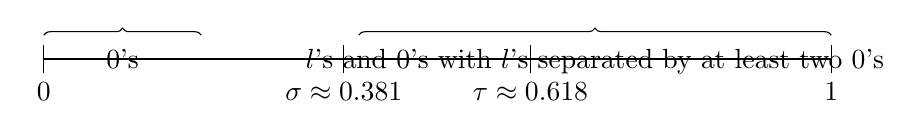
\begin{tikzpicture}
\draw(0,0)--(10,0);
\draw(0,5pt)--(0,-5pt) node[below] {$ 0 $};
\draw(3.81,5pt)--(3.81,-5pt) node[below] {$ \sigma \approx 0.381 $};
\draw(6.18,5pt)--(6.18,-5pt) node[below] {$ \tau \approx 0.618 $};
\draw(10,5pt)--(10,-5pt) node[below] {$ 1 $};
\draw[decorate, decoration={brace}, yshift=2ex]  (0,0) -- node[below=0.4ex] {$0$'s}  (2,0);
\draw[decorate, decoration={brace, mirror}, yshift=2ex]  (10,0) -- node[below=0.4ex] {$l$'s and $0$'s with $l$'s separated by at least two $0$'s}  (4,0);
\end{tikzpicture}


Let now \( [a_0, b_0] = [a, b] \) and define 
\[
    \begin{split}
        x_k & = b_k - \tau (b_k - a_k) \\ 
        y_k & = a_k + \tau (b_k - a_k)
    \end{split}
\]
and
\[  
    [a_{k + 1}, b_{k + 1}] = 
        \begin{cases}
            [a_k, y_k] & \text{ if } f(x_k) < f(y_k)  \\
            [x_k, b_k] & \text{ if } f(x_k) \ge f(y_k)
        \end{cases}
\]
It follows that \( [a_k, b_k] \supset [a_{k + 1}, b_{k + 1}] \) is a decreasing series of intervals with
\[  
    (b_{k + 1} - a_{k + 1}) =  \tau(b_k - a_k)
\]
where the interval converges to \( \xi \). This leads to the following algorithm:
\bigskip


\begin{algorithm}[Golden Section Search]\label{algo:golden_section_search}
\end{algorithm}
\inputminted[fontsize=\small, framesep=0.35cm, frame=lines, python3=true]{python}{golden_section.py}
\bigskip

\begin{tikzpicture}
\begin{axis}[axis lines=left, xlabel=$x$, ylabel={$f(x)$}, xmin=-5, xmax=5, ymin=0, ymax=5]
\addplot[domain=-10:10,samples=100,color=red]{(x - 2)^2 + 1};
\addlegendentry{$ {(x - 2)}^2 + 1 $}
\addplot[domain=-10:10, samples=100, color=blue]{x^2};
\addlegendentry{$ x^2 $}
\end{axis}
\end{tikzpicture}
